\documentclass[a4paper]{article}

%% Language and font encodings
\usepackage[english]{babel}
\usepackage[utf8x]{inputenc}
\usepackage[T1]{fontenc}

%% Sets page size and margins
\usepackage[a4paper,top=3cm,bottom=2cm,left=3cm,right=3cm,marginparwidth=1.75cm]{geometry}

%% Useful packages
\usepackage{amsmath}
\usepackage{graphicx}
\usepackage[colorinlistoftodos]{todonotes}
\usepackage[colorlinks=true, allcolors=blue]{hyperref}

\title{Reporte de Actividad 4\\Introducción a la programación de los intérpretes de comandos}
\author{Michelle Contreras Cossio}
\date{21 de Febrero del 2018}

\begin{document}
\maketitle

\section{Introducción} 
En el siguiente reporte resume los resultados obtenidos al realizar la Actividad \#4 de la clase de Física Computacional 1. En esta tenemos una introducción a "Shell", donde usamos y definimos sus comandos principales y aprendemos a escribir scripts que automatizan algunas acciones. Además, se realizó una síntesis del tutorial "Shell Scripting Tutorial", escrito por Steve Parker. 

\section{Fundamentos}

El sistema operativo Linux, con el cual trabajamos en el centro de cómputo, utiliza un intérprete de comandos, llamado Shell,el interprete de comandos es el programa que recibe lo que se escribe en la terminal y lo convierte en instrucciones para el sistema operativo. \\
 
Existe una gran variedad de intérpretes de comandos, como son:  C Shell (/bin/csh), Bourne Shell (/bin/sh), Korn Shell (/bin/ksh/), Bourne Again Shell (/bin/bash), y otros. En este caso trabajemos con /bin/bash/ y /bin/sh (Bourne Again Shell y Bourne Shell, respectivamente). \\

Como se mencionó, trabajaremos con scripts, un script, archivo de órdenes, archivo de procesamiento por lotes que por lo regular se almacena en un archivo de texto plano. El uso habitual de los guiones es realizar diversas tareas como combinar componentes, interactuar con el sistema operativo o con el usuario. 

\section{Resumen de Comandos}

\begin{itemize}
\item \textbf{cat}: Lee archivos y los muestra en pantalla (pero los muestra rápidamente, no es para la lectura del usuario), puede además concatenarlos en un solo archivo de salida. 
\item \textbf{chmod}: Este comando permite cambiar los permisos de acceso (leer, editar, ejecutar), sobre el archivo, por parte del dueño, del grupo de usuarios registrados y de cualquier usuario en general.
\item \textbf{echo}: Es un comando para la impresión de un texto en pantalla. Es comúnmente utilizado dentro de scripts
\item\textbf{grep}: Significa global regular expression print, es usado para buscar la ubicación o renglones que contengan cierta cadena de texto dentro de un archivo y las muestr. 
\item \textbf{less}: Permite ver, de manera detallada, el contenido de un archivo, pero no editarlo. 
\item \textbf{ls}: Enlista el contenido (archivos o directorios) que se tiene en el directorio asignado. Al añadirle la bandera "-alg", nos permite ver los permisos de acceso que se tienen sobre los archivos. 
\item \textbf{wc}: Realiza un conteo, de palabras, caracteres o saltos de línea, del archivo indicado. 
\item \textbf{Redirectores: |, >}: El símbolo "|" crea "pipes", que conectan dos comandos, donde la salida de un programa es la entrada del otro. Por otro lado, el caracter ">" redirecciona la salida de un comando ejecutado a un archivo que se creará. 
\end{itemize}


\section{Actividad Realizada}

En esta sección se añade la actividad que se realizó para conocer los comandos principales del shell. 

\begin{enumerate}
\item Se inició utilizando un script proporcionado y adecuándolo a la estación de sondeos atmosféricos con la que trabajamos la semana pasada, la cual fue del Aeropuerto Internacional de Adelaida, en Australia.
\item Posteriormente, se utilizó el comando ls -alg para observar los permisos con los que contaba este archivo. 
\begin{figure}[h!]
  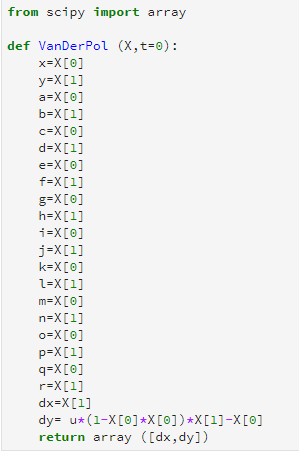
\includegraphics[width=8cm]{1.png}
  \centering
  \label{fig:1}
\end{figure}
\item Al no ser un archivo ejecutable, se cambió el permiso con el comando chmod y se procedió a ejecutar el script, el cual descargó 12 archivos (uno por mes) de la base de datos de la universidad de Wyoming. 
\begin{figure}[h!]
  
\includegraphics[width=8cm]{2.png}
  \centering
  \label{fig:2}
\end{figure}
\begin{figure}[h!]
  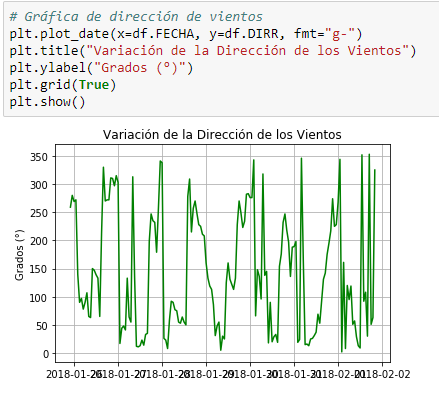
\includegraphics[width=13cm]{3.png}
  \centering
  \label{fig:3}
\end{figure}
\item El comando less permitió observar con detenimiento un archivo. El comando cat, en cambio, lo mostró más rápido. 
\item El comando grep permitió buscar renglones
\begin{figure}[h!]
  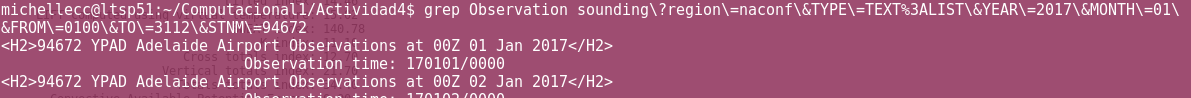
\includegraphics[width=12cm]{4.png}
  \centering
  \label{fig:4}
\end{figure}
\item El comando file nos dejó ver el tipo de archivo que eran los archivos descargados con el script.
\begin{figure}[h!]
  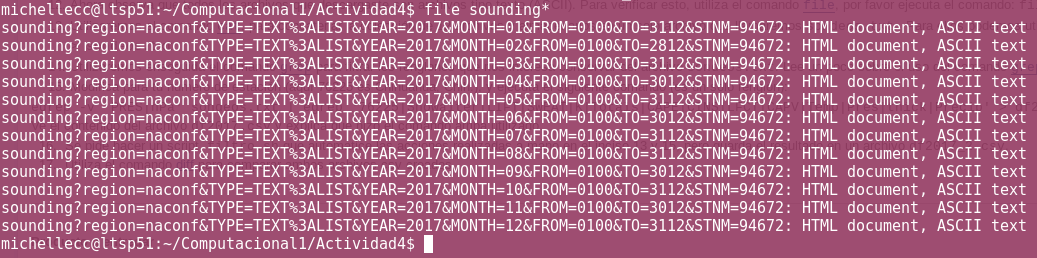
\includegraphics[width=9cm]{5.png}
  \centering
  \label{fig:5}
\end{figure}
\item El comando cat se utilizó nuevamente para juntar los 12 archivos en uno txt. Con:
\begin{verbatim}
cat sounding* > sondeos.txt
\end{verbatim}
\begin{figure}[h!]
  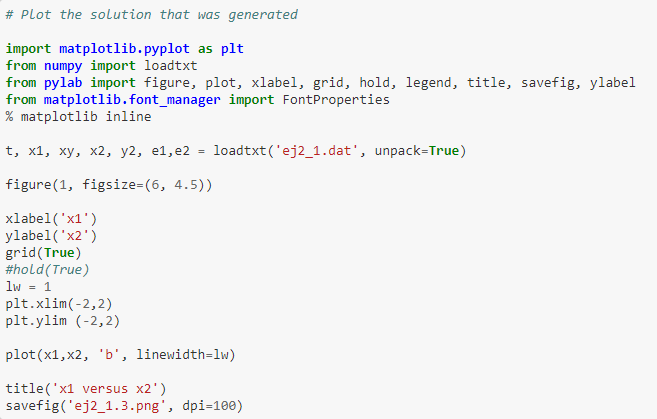
\includegraphics[width=10cm]{6.png}
  \centering
  \label{fig:6}
\end{figure}
\item Posteriormente, se utilizó el siguiente comando (en una sola linea): 
 \begin{verbatim}
 egrep -v 'PRES|hPa' sondeos.txt | egrep '94672|Showalter|LIFT|SWEAT|K|Totals
 |CAPE|CINS|LFCT|CAPV|Temp|Pres|thick|Precip' > df2017.csv
 \end{verbatim}
 \begin{figure}[h!]
  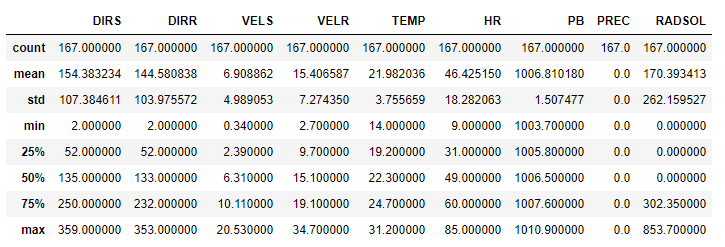
\includegraphics[width=8cm]{7.png}
  \centering
  \label{fig:7}
\end{figure}
El cual retira los renglones que empiecen con 'PRES$|$hPa' del archivo creado en el paso 7. Posteriormente dejaba únicamente los renglones que comenzaban con alguna de las siguentes opciones: '94672|Showalter|LIFT|SWEAT|K|Totals|CAPE|CINS|LFCT|CAPV|Temp|Pres|thick| Precip' y el resultado lo mandó al archivo df2017.csv.
\begin{figure}[h!]
  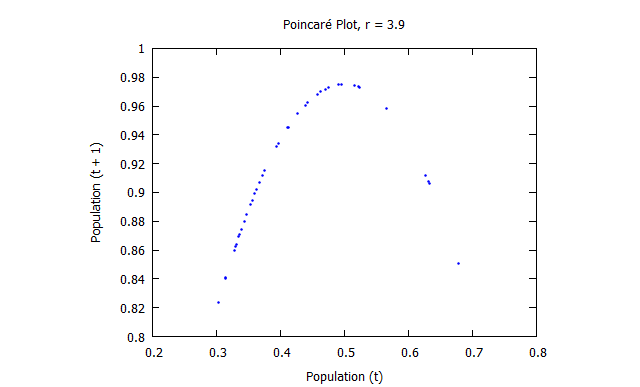
\includegraphics[width=7.5cm]{8.png}
  \centering
  \label{fig:8}
\end{figure}
 \item Se creó un script que automatizara el paso 7 y 8, creando un archivo llamado df2017\_2.csv. Estos fueron comparados con el comando diff, verificando que no existiera ninguna diferencia entre ambos.
 \begin{figure}[h!]
  
\includegraphics[width=8cm]{9.png}
  \centering
  \label{fig:9}
\end{figure}
\begin{figure}[h!]
  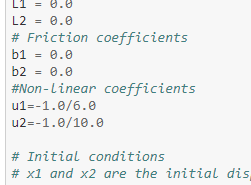
\includegraphics[width=7.5cm]{10.png}
  \centering
  \label{fig:10}
\end{figure}
\begin{figure}[h!]
  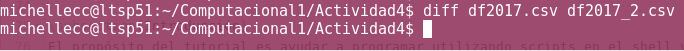
\includegraphics[width=10cm]{11.png}
  \centering
  \label{fig:11}
\end{figure}
\end{enumerate}


\section{Síntesis de "Shell Scripting Tutorial"}

\textbf{NOTA:} Todos los scripts creados como ejemplos se anexan en la carpeta "Scripts", con la misma numeración aquí mencionada. 

\subsection{Introducción}
El propósito del tutorial es ayudar a programar utilizando scripts en el shell y enseñar lo básico por medio de ejemplos y ejercicios. No obstante, el tutorial no es para cualquier individuo, este asume conocimiento básico del uso del Shell, de programación y comandos de unix. 
Bourne Shell fue creado por Steve Bourne, este y el Bourne Again Shell son los que cubre el tutorial, sin embargo, existen otros como Korn Shell (ksh), C Shell (csh), entre otros.\\
\\
\textbf{Script \#1:} 

Se creó un script usando los siguientes comandos:
\begin{verbatim}
echo '#!/bin/sh' > my-script.sh
echo 'echo Hello World' >> my-script.sh
\end{verbatim}

Que obtuvo como salida:
\begin{figure}[h!]
  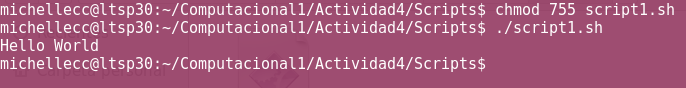
\includegraphics[width=10cm]{script1.jpg}
  \centering
  \label{fig:12}
\end{figure}

\subsection{Filosofía}
La programación de Shell Scripts tiene un poca mala fama, debido a la que no es tan veloz, en comparación con C  o Perl; la otra razón importante es que no es tan estricto con su sintaxis, lo que provoca que existan scripts con poca calidad.

Los criterios que se toman en cuenta para calificar un script como bueno, son: que tenga un diseño claro y legible, y que se evite el uso de comandos innecesarios, ya que esto provoca lentitud. 

Sin embargo, cuando estos criterios se toman en cuenta al escribir el script, se tienen ciertas ventajas. Por ejemplo, que el diseño sea claro y legible permite que siga creciendo el script y que lo pueda mantener cualquier usuario, no solo el autor. 

Algunas debilidades de la programación por Shell Scripting es que no se hace muy buen uso de la indentación y resultan más difíciles de leer. Por otro lado, otra debilidad, es que hay diferentes maneras de realizar una misma acción, sin embargo, a veces una es más eficiente que la otra, y si bien es cierto, si queremos realizar solo una acción, no es tan significativo, el problema se registra cuando la tenemos dentro de un ciclo. 

Como recomendación, se añade que es necesario saber que los shell scripts siempre son susceptibles a errores y es importante siempre pedir retroalimentación cuando lo compartes.

\subsection{Primer Script}
\textbf{Script \#2:}
\begin{verbatim}
#!/bin/sh
# Comentario
echo Hello World 
\end{verbatim}

La primera línea indica que el archivo se ejecuta con /bin/sh, es decir el Bourne Shell. La segunda linea empieza con \#, que indica un comentario y se ignora lo que incluya ese renglón, a excepción del primer renglón que se empieza con \#!, que indica que se debe interpretar lo que siga por el Bourne Shell.

La tercera línea muestra al comando echo con dos parámetros "Hello" y "World", echo pone automáticamente espacio entre los parámetros.

En la terminal se utiliza el comando chmod para cambiar los permisos sobre el archivo y permitir ejecutarlo, posteriormente se ejecuta: 
\begin{figure}[h!]
  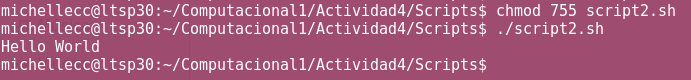
\includegraphics[width=10cm]{script2.png}
  \centering
  \label{fig:13}
\end{figure}

Es necesario diferenciar como funciona el comando echo, si se agregaran espacios a la línea de código \textit{echo Hello    World}, daría la misma salida que en la imagen anterior. Por otro lado, si se da la orden: \textit{echo "Hello    World"}, el resultado si nos daría los espacios exactamente como los ingresamos, esto debido a que pasa la cadena como un solo parámetro. \\
\\
\textbf{Script \#3:}
\begin{verbatim}
#!/bin/sh
#Comentario
echo "Hello      World"
echo "Hello World"
echo "Hello * World"
echo Hello * World
echo Hello      World
echo "Hello" World
echo Hello "     " World
echo "Hello "*" World"
echo `hello` world
echo 'hello' world
\end{verbatim}

Y dio como resultado, que permite diferenciar entre como deben ser ingresados los parámetros para que nos de el resultado que queramos: 
\begin{figure}[h!]
  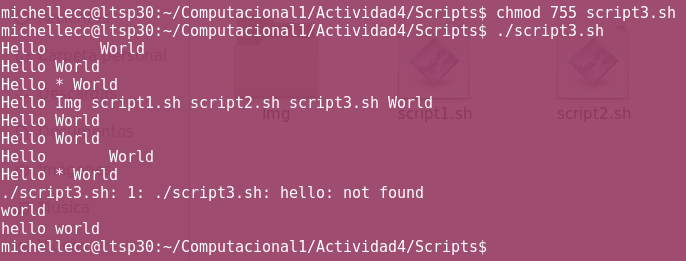
\includegraphics[width=10cm]{script3.png}
  \centering
  \label{fig:14}
\end{figure}

\subsection{Variables (parte 1)}

Como en todo lenguaje de programación, se tienen variables, a las cuales se les puede asignar valor y manipular su contenido. 

Para que las variables funcionen, no deben existir espacios al momento de asignarles valor, es decir: VAR=value\\
\\
\textbf{Script \#4:}

\begin{verbatim}
#!/bin/sh
MY_MESSAGE="Hello World"
echo $MY_MESSAGE
\end{verbatim}

Este script da el mismo resultado que los anteriores con los que hemos estado trabajando, sin embargo, este asigna a la variable "MY\_MESSAGE" la cadena "Hello World", posteriormente lo imprime a la pantalla. Es necesario añadir que las variables solo admite un parámetro, por lo que si se tienen varias palabras, se deben poner entre comillas.
\begin{figure}[h!]
  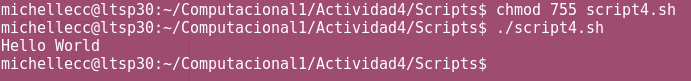
\includegraphics[width=10cm]{script4.png}
  \centering
  \label{fig:15}
\end{figure}

El shell permite que las variables sean de cualquier tipo, cadenas, enteros, reales. De hecho, todos los guarda como cadenas, así que si se busca operar con estas, no se podrá. 

También se puede obtener el valor de las variables desde el usuario, usando el comando read.

Las variables en el Bourne Shell no necesitan ser declaradas, sin embargo, si se utiliza una variable que no está declarada, no marcará error, solo estará vacía, esto puede causar muchos errores. Para arreglar un poco eso existe el comando \textit{export}, que, como su nombre lo dice, exporta la variable por otro programa y permite darle valor(momentáneo) a la variable desde fuera. Otra opción es al ejecutar el archivo poner ". ./".\\
\\
\textbf{Script \#5:} Otra cosa que se puede hacer con las variables es usarlas como nombre de archivo, notese que se deben agregar llaves, ya que se añade "\_file" al nombre de la variable: 
\begin{verbatim}
#!/bin/sh
echo "What is your name?"
read USER_NAME
echo "Hello $USER_NAME"
echo "I will create you a file called ${USER_NAME}_file"
touch "${USER_NAME}_file"
\end{verbatim}

Que da como resultado: 
\begin{figure}[h!]
  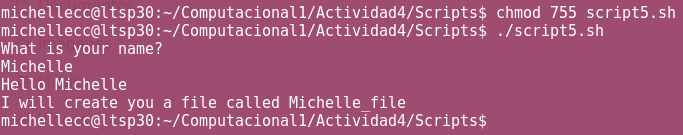
\includegraphics[width=10cm]{script5.png}
  \centering
  \label{fig:16}\\
\end{figure}
\\
\\
\\
\\
Y crea el archivo:
\begin{figure}[h!]
  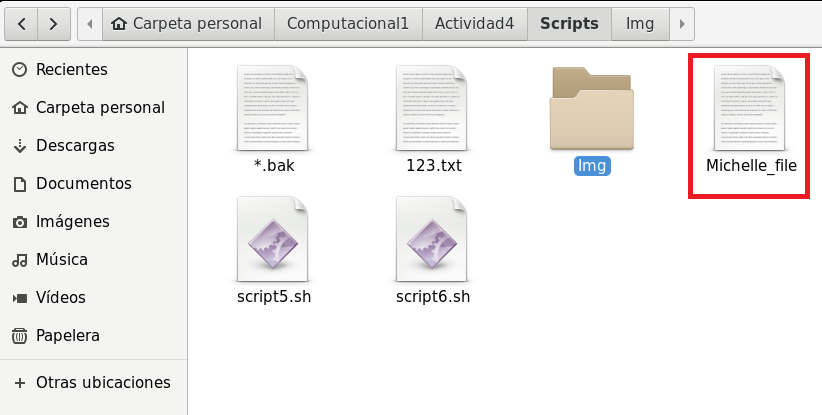
\includegraphics[width=10cm]{script5_1.png}
  \centering
  \label{fig:17}
\end{figure}

\subsection{Wildcards}
En español se conocen como \textit{caracteres comodín}. \\
\\
\textbf{Script \#6:}

\begin{verbatim}
#/bin/sh
cp /home/michellecc/Computacional1/Actividad4/Scripts/ *.txt/home/michellecc
/Computacional1/Actividad4/Scripts/Img
\end{verbatim}

Este script mueve los archivos txt encontrados en el primer directorio, al segundo:
\begin{figure}[h!]
  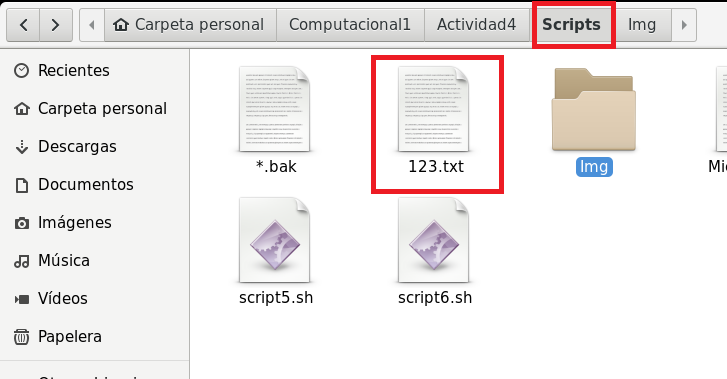
\includegraphics[width=9cm]{script6.png}
  \centering
  \label{fig:18}
\end{figure}
\begin{figure}[h!]
  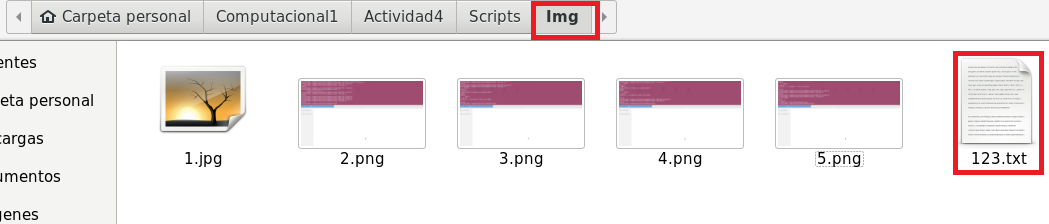
\includegraphics[width=9cm]{script6_1.png}
  \centering
  \label{fig:19}
\end{figure}

\textbf{Script \#7:}
\begin{verbatim}
#!/bin/sh
files=`ls -1 *.txt`
for f in *.txt; do
mv "$f" "$(basename "$f" .txt).bak"
done
\end{verbatim}

Este script convierte a todos los archivos txt en bak:
\begin{figure}[h!]
  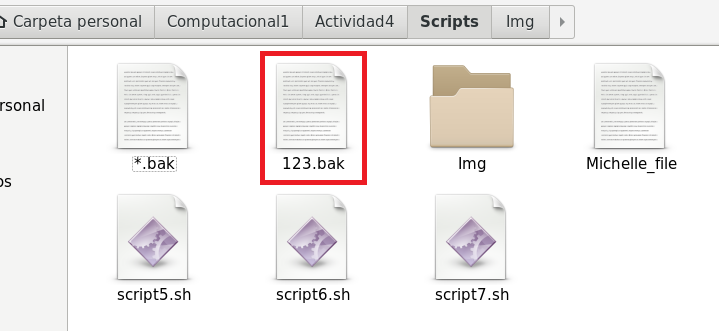
\includegraphics[width=9cm]{script7.png}
  \centering
  \label{fig:20}
\end{figure}

\subsection{Secuencias de escape}
Existen algunos caracteres que ya tienen funciones dentro del Shell, por ejemplo, las comillas " sirven para formar cadenas, el asterisco * muestra los archivos dentro del directorio, el signo de pesos \$ llama a alguna variable, entre otros. El problema surge cuando queremos usar esos caracteres pero no para su función dentro del shell, solo como caracteres. Para ello se usa el backslash $\backslash$. \\
\\
\textbf{Script \#8}: Se muestran las diferencias al trabajar con el asterisco: 
 \begin{verbatim}
#/bin/sh
echo *
echo *txt
echo "*"
echo "*txt"
 \end{verbatim}

Que tiene como salida:
\begin{figure}[h!]
  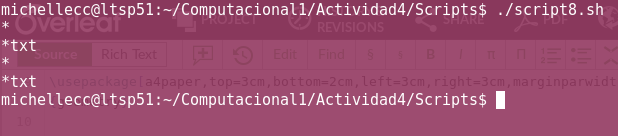
\includegraphics[width=10cm]{script8.png}
  \centering
  \label{fig:21}
\end{figure}

\textbf{Script \#9}: Se muestra como se utiliza el backslash para poder usar los caracteres mencionados:
 \begin{verbatim}
#/bin/sh
echo "A quote is \", backslash is \\, backtick is \`."
echo "A few spaces are    ; dollar is \$. \$X is ${X}."
 \end{verbatim}
Que tiene como salida:
 \begin{figure}[h!]
  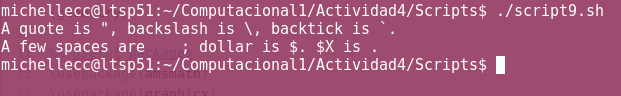
\includegraphics[width=10cm]{script9.png}
  \centering
  \label{fig:22}
\end{figure}

\subsection{Ciclos}

Los ciclos o "loops" son comunes en los lenguajes de programación, para repetir cierta tarea una cierta cantidad de veces. Los loops que maneja el Bourne shell son for y while.\\
\\

\begin{itemize}
\item \textbf{For loops:} Estos iteran en valores ya establecidos hasta que la lista se acaba, sin importar si son números o cualquier entrada que se le de. \\
\\
\textbf{Script \#10:} 
\begin{verbatim}
#!/bin/sh
for i in hello 1 * 2 goodbye 
do
  echo "Looping ... i is set to $i"
done
\end{verbatim}

Que da como salida:
 \begin{figure}[h!]
  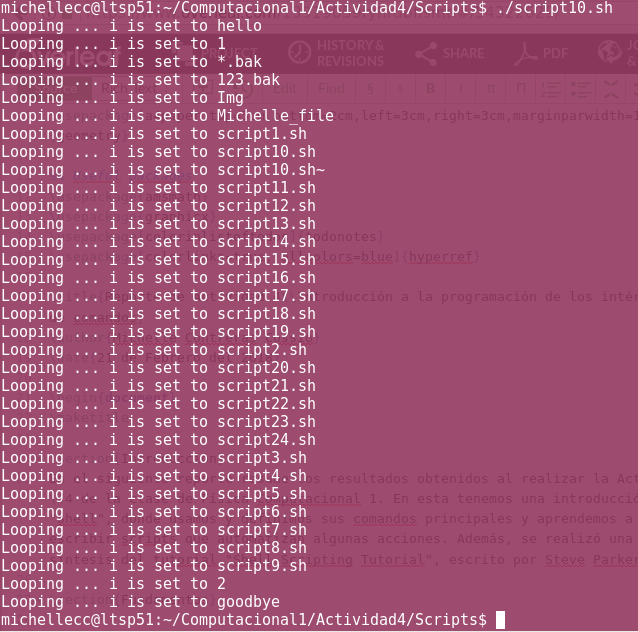
\includegraphics[width=8cm]{script10.png}
  \centering
  \label{fig:23}
\end{figure}

\item \textbf{While Loops:} Estos tienen una condición de salida y hasta que esa se cumpla, el ciclo se acaba, aunque tambien se puede salir de ellos con el comando \textit{ctrl+c}.\\
\\
\textbf{Script \#11:} 
\begin{verbatim}
#!/bin/sh
INPUT_STRING=hello
while [ "$INPUT_STRING" != "bye" ]
do
  echo "Please type something in (bye to quit)"
  read INPUT_STRING
  echo "You typed: $INPUT_STRING"
done
\end{verbatim}

Da como salida:
 \begin{figure}[h!]
  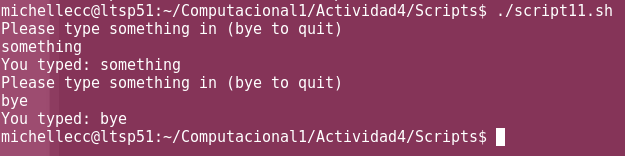
\includegraphics[width=10cm]{script11.png}
  \centering
  \label{fig:24}
\end{figure}
\end{itemize}

\subsection{Test}
Test se llama haciendo uso de "[", y es como un programa por sí solo. Este es parte de la estructura del if (elif y else se pueden omitir):
\begin{verbatim}
if  [ something ]; then
 echo "Something"
 elif [ something_else ]; then
   echo "Something else"
 else
   echo "None of the above"
fi
\end{verbatim}

El constructo if realiza una acción dependiendo si lo que se encuentra dentro de los corchetes es cierto. 

Es necesario agregar que el punto y coma se utiliza para unir dos lineas en un solo renglón. El backslash $\backslash$ se usa para indicar que no es el final de la línea y que el siguiente renglón se debe usar como continuación de la línea.

En lugar de if se puede usar \&\& o $||$, que producirán un segmento de código si el comando es verdadero o falso, respectivamente. \\
\\
\textbf{Script \#12:} Este script ejemplifica lo anteriormente mencionado
\begin{verbatim}
#!/bin/sh
X=5
if [ "$X" -lt "0" ]
then
  echo "X is less than zero"
fi
if [ "$X" -gt "0" ]; then
  echo "X is more than zero"
fi
[ "$X" -le "0" ] && \
      echo "X is less than or equal to  zero"
[ "$X" -ge "0" ] && \
      echo "X is more than or equal to zero"
[ "$X" = "0" ] && \
      echo "X is the string or number \"0\""
[ "$X" = "hello" ] && \
      echo "X matches the string \"hello\""
[ "$X" != "hello" ] && \
      echo "X is not the string \"hello\""
[ -n "$X" ] && \
      echo "X is of nonzero length"
[ -f "$X" ] && \
      echo "X is the path of a real file" || \
      echo "No such file: $X"
[ -x "$X" ] && \
      echo "X is the path of an executable file"
[ "$X" -nt "/etc/passwd" ] && \
      echo "X is a file which is newer than /etc/passwd"
\end{verbatim}

Con salida:
 \begin{figure}[h!]
  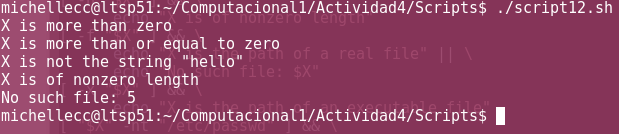
\includegraphics[width=10cm]{script12.png}
  \centering
  \label{fig:25}
\end{figure}

Tambien el test se puede usar para ciclos while: \\
\\
\textbf{Script \#13:} Este ciclo se repetirá hasta que lo que está en el test se cumpla.
\begin{verbatim}
#!/bin/sh
X=0
while [ -n "$X" ]
do
  echo "Enter some text (RETURN to quit)"
  read X
  echo "You said: $X"
done
\end{verbatim}

Con salida:
 \begin{figure}[h!]
  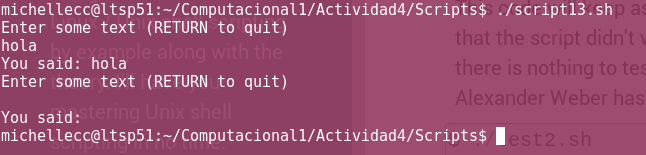
\includegraphics[width=8cm]{script13.png}
  \centering
  \label{fig:26}
\end{figure}


\subsection{Case}
Como en otros lenguajes de programación, el case es un conjunto de if/then/else y funciona exactamente igual; escoge una variable y la compara con opciones (o casos) de posibles valores de la variable y de no ser así, la opción default "*)" contiene todos los casos no listados.  
Para iniciar un case se pone case y la variable a evaluar. Para terminarlo se pone esac (case al revés).\\
\\
\textbf{Script \#14:} El script muestra un case dentro de un while.
\begin{verbatim}
#!/bin/sh
echo "Please talk to me ..."
while :
do
  read INPUT_STRING
  case $INPUT_STRING in
	hello)
		echo "Hello yourself!"
		;;
	bye)
		echo "See you again!"
		break
		;;
	*)
		echo "Sorry, I don't understand"
		;;
  esac
done
echo 
echo "That's all folks!"
\end{verbatim}

Y esta es su salida:
 \begin{figure}[h!]
  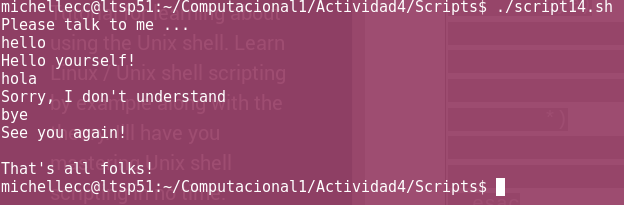
\includegraphics[width=8cm]{script14.png}
  \centering
  \label{fig:27}
\end{figure}

\subsection{Variables (parte 2)}
Existen variables que ya tienen valor, unas pocas son:
\begin{itemize}
\item \textbf{\$0:} nombre del programa donde se ubica.
\item \textbf{\$1:} nombre del primer parámetro.
\item \textbf{\$2:} nombre del segundo parámetro.
\item \textbf{\$3...9:} nombre del (número) parámetro.
\item \textbf{\$@:} nombre de todos los parámetros.
\item \textbf{\$\#:} número de parámetros que contiene.
\item \textbf{\$?:} el status de salida del último comando.
\item \textbf{\$\$:} PID (Process IDentifier), identificador de proceso del shell que esta corriendo. 
\item \textbf{\$!:} PID del último proceso en el fondo. 
\end{itemize}

(Los últimos tres comandos no me quedaron muy claros)\\
\\
\textbf{Script \#15:} 
\begin{verbatim}
#!/bin/sh
echo "I was called with $# parameters"
echo "My name is $0"
echo "My first parameter is $1"
echo "My second parameter is $2"
echo "All parameters are $@"
\end{verbatim}

Y su salida es:
 \begin{figure}[h!]
  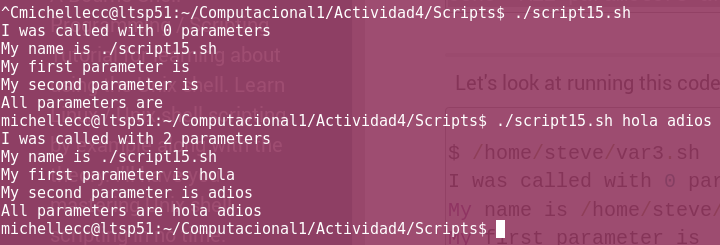
\includegraphics[width=8.5cm]{script15.png}
  \centering
  \label{fig:28}
\end{figure}

Una última variable importante es IFS que por sus siglas en inglés es Internal Field Separator, se podría considerar como un separador de variables, el siguiente script lo ejemplifica mejor:\\
\\
\textbf{Script \#16:}
\begin{verbatim}
#!/bin/sh
old_IFS="$IFS"
IFS=:
echo "Please input some data separated by colons ..."
read x y z
IFS=$old_IFS
echo "x is $x y is $y z is $z"
\end{verbatim}

Su salida es:
 \begin{figure}[h!]
  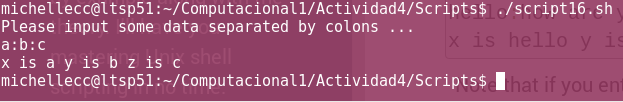
\includegraphics[width=9cm]{script16.png}
  \centering
  \label{fig:29}
\end{figure}
\subsection{Variables (parte 3)}
Las llaves se usan para evitar confusiones en las variables, por ejemplo: \\
\\
\textbf{Script \#17:}
\begin{verbatim}
#!/bin/sh
foo=sun
echo $fooshine     
echo ${foo}shine   
\end{verbatim}

Que tiene como salida lo siguiente, donde se observa la diferencia, la variable fooshine no se encuentra definida y no da valor, por otro lado, al agregarle las llaves, nos despliega la palabra sunshine. :
 \begin{figure}[h!]
  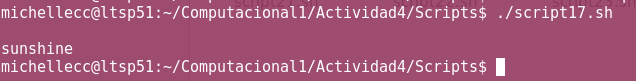
\includegraphics[width=10cm]{script17.png}
  \centering
  \label{fig:30}
\end{figure}

\textbf{Script \#18:} El siguiente código nos da un valor default en caso de que no se ingrese un nombre por el usuario: 
\begin{verbatim}
#!/bin/sh
echo -en "What is your name [ `whoami` ] "
read myname
echo "Your name is : ${myname:-`whoami`}"
\end{verbatim}

Con el símbolo ":-" estamos dándole un valor default a la variable, en caso de que el usuario no ingrese uno, su salida es:
\begin{figure}[h!]
  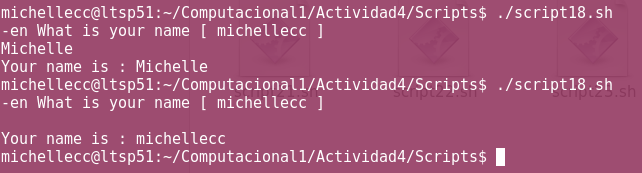
\includegraphics[width=10cm]{script18.png}
  \centering
  \label{fig:31}
\end{figure}

\subsection{Programas externos}
Son comandos de Unix que se usan en el shell. Algunos ejemplos son echo, which, test, tr, grep, expr, cut. 

Para hablar de comandos externos se utiliza la comilla invertida (`). Esta nos indica que el texto encerrado dentro se ejecutará como comando, un ejemplo:\\
\\
\textbf{Script \#19:}
\begin{verbatim}
#!/bin/sh
MYNAME=`grep "^${USER}:" /etc/passwd | cut -d: -f5`
echo $MYNAME
\end{verbatim}

Que tiene como salida:
 \begin{figure}[h!]
  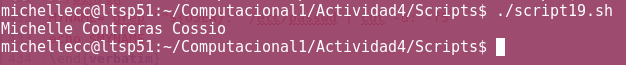
\includegraphics[width=10cm]{script19.png}
  \centering
  \label{fig:32}
\end{figure}

\textbf{Script \#20:}
\begin{verbatim}
#!/bin/sh
MYNAME=`grep "^${USER}:" /etc/passwd | cut -d: -f5`
echo $MYNAME
\end{verbatim}

Con salida: 
\begin{figure}[h!]
  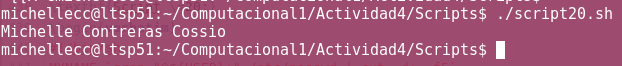
\includegraphics[width=10cm]{script20.png}
  \centering
  \label{fig:33}
\end{figure}


\subsection{Funciones}
Programar scripts con Bourne shell nos da la opción de crear funciones, ya sea con un simple script, declarando la funciom en el archivo donde se manda o con el comando de library.

En shell no existe diferencia entre procedures y funciones, una función en shell puede ser cualquiera de las dos o las dos. Las funciones dan un valor de cuatro maneras diferentes: 
\begin{itemize}
\item Cambia el estado de una o muchas variables. 
\item Usa el comando exit para terminar el script.
\item Usa el comando return para terminar la función y regresa el valor a la sección de donde fue llamada.
\item echo output a stdout (estándar output).
\end{itemize}

Un ejemplo de función: \\
\\ 
\textbf{Script \#21:}
\begin{verbatim}
#!/bin/sh
# A simple script with a function...

add_a_user()
{
  USER=$1
  PASSWORD=$2
  shift; shift;
  # Having shifted twice, the rest is now comments ...
  COMMENTS=$@
  echo "Adding user $USER ..."
  echo useradd -c "$COMMENTS" $USER
  echo passwd $USER $PASSWORD
  echo "Added user $USER ($COMMENTS) with pass $PASSWORD"
}

###
# Main body of script starts here
###
echo "Start of script..."
add_a_user bob letmein Bob Holness the presenter
add_a_user fred badpassword Fred Durst the singer
add_a_user bilko worsepassword Sgt. Bilko the role model
echo "End of script..."
\end{verbatim}

Su salida es:
\begin{figure}[h!]
  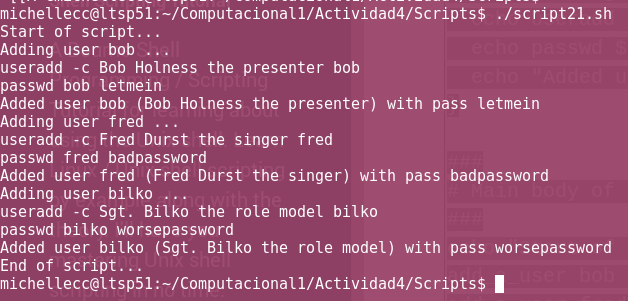
\includegraphics[width=8cm]{script21.png}
  \centering
  \label{fig:34}
\end{figure}

Para declarar la variable se utiliza () al final del renglón. Seguido por llaves, donde todo lo que estas encierran es el código de la función. Este código no correrá hasta que se llame la función, en el ejemplo, esto ocurre hasta que el script inicia. 

Existen variables globales, que pueden usarse tanto en el script principal como en la función y esta puede cambiar su valor, al menos que se le restrinja hacerlo, usando un subshell. Sin embargo, no puede cambiar los parámetros con los que fue llamada, al menos que los asigne a una variable, esa si la puede manipular.

Otra propiedad de las variables es que pueden ser recursivas, es decir, que se llame a si misma. Un ejemplo es con la función factorial: \\
\\
\textbf{Script \#22:}
\begin{verbatim}
#!/bin/sh

factorial()
{
  if [ "$1" -gt "1" ]; then
    i=`expr $1 - 1`
    j=`factorial $i`
    k=`expr $1 \* $j`
    echo $k
  else
    echo 1
  fi
}


while :
do
  echo "Enter a number:"
  read x
  factorial $x
done
\end{verbatim}

Y esta nos regresa el factorial de un número ingresado:
 \begin{figure}[h!]
  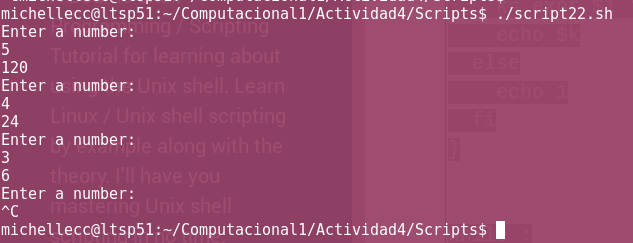
\includegraphics[width=8cm]{script22.png}
  \centering
  \label{fig:35}
\end{figure}

Como fue mencionado con anterioridad, también se pueden crear funciones con librerías. estas lo que hacen es separar la función en otro archivo con extensión .lib y al llamarla desde un script, se le llama como un archivo ejecutable, básicamente lo que hace es separar en múltiples archivos, para poder usarla en más de un script.

\subsection{Tips y consejos}
En esta sección se ven algunos consejos rápidos y básicos para mejorar la redacción de scripts. 

Existen algunos comandos importantes, como grep (definido en la sección 3), cut que remueve lineas o pedazos de algun archivo; otro es tr que cambia o sustituye un set de caracteres en otro.

Otro tip es hacer trampa (cheating), esto es para poder remediar cosas que el shell no hace bien. Existen dos formas de cheating, con sed o con awk. 

La función awk es que encuentra y reemplaza texto. Por su parte, sed elimina o sustituye cadenas o líneas, similar a grep, pero grep borra las líneas completas. 

Telnet es otro truco que se usa, aquí dos ejemplos:\\
\\
\textbf{Script \# 23:}
\begin{verbatim}
#!/bin/sh
host=127.0.0.1
port=23
login=steve
passwd=hellothere
cmd="ls /tmp"

echo open ${host} ${port}
sleep 1
echo ${login}
sleep 1
echo ${passwd}
sleep 1
echo ${cmd}
sleep 1
echo exit
\end{verbatim}

Con salida: 
 \begin{figure}[h!]
  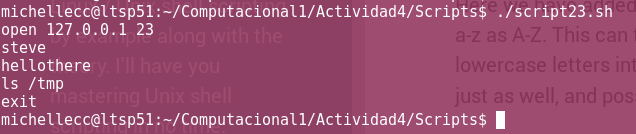
\includegraphics[width=10cm]{script23.png}
  \centering
  \label{fig:36}
\end{figure}

\textbf{Script \#24:}
\begin{verbatim}
#!/bin/sh
# telnet2.sh | telnet > FILE1 
host=127.0.0.1
port=23
login=steve
passwd=hellothere
cmd="ls /tmp"
timeout=3
file=file1
prompt="$"

echo open ${host} ${port}
sleep 1
tout=${timeout}
while [ "${tout}" -ge 0 ]
do
    if tail -1 "${file}" 2>/dev/null | egrep -e "login:" > /dev/null
    then
        echo "${login}"
        sleep 1
        tout=-5
        continue
    else
        sleep 1
        tout=`expr ${tout} - 1`
    fi
done

if [ "${tout}" -ne "-5" ]; then
  exit 1
fi

tout=${timeout}
while [ "${tout}" -ge 0 ]
do
    if tail -1 "${file}" 2>/dev/null | egrep -e "Password:" > /dev/null
    then
        echo "${passwd}"
        sleep 1
        tout=-5
        continue
    else
      if tail -1 "${file}" 2>/dev/null | egrep -e "${prompt}" > /dev/null
      then
        tout=-5
      else
        sleep 1
        tout=`expr ${tout} - 1`
      fi
    fi
done

if [ "${tout}" -ne "-5" ]; then
  exit 1
fi

> ${file}

echo ${cmd}
sleep 1
echo exit
\end{verbatim}

Con salida:
 \begin{figure}[h!]
  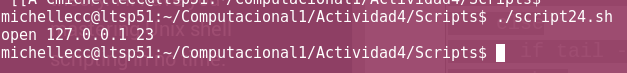
\includegraphics[width=10cm]{script24.png}
  \centering
  \label{fig:37}
\end{figure}

\subsection{Guía rápida de comandos}
Esta guía resume algunos comandos, no tan triviales, y que considero que serán de nuestro uso en la redacción de scripts: 

\begin{tabbing}
\hspace*{2cm} \= \hspace*{5cm} \kill
Comando \> Descripción \\
\ \& \> Corre el comando anterior en el fondo. \\
\ \&\& \> AND Lógico\\
\ $||$ \> OR Lógico\\
\ \^~ \> Inicio de la línea\\
\ \$ \> Final de la línea\\
\ \textbf{=} \> Igualdad de cadenas \\
\ ! \> NOT lógico \\
\ \$0 \> Nombre del comando actual \\
\ \$1 \> Nombre del argumento del comando actual \\
\ $-$eq \> Igualdad numérica \\
\ $-$ne \> Desigualdad numérica \\
\ $-$lt \> Menor que \\
\ $-$le \> Menor o igual que \\
\ $-$gt \> Mayor que que \\
\ $-$ge \> Mayor o igual que \\
\ $-$nt \> Más nuevo que \\
\ $-$d \> Directorio \\
\ $-$f \> Archivo \\
\ $-$r \> Archivo legible \\
\ $-$w \> Archivo editable\\
\ $-$x \> Archivo ejecutable \\
\end{tabbing}

\subsection{Shells interactivos}
\begin{itemize}
\item \textbf{bash:} 

Cuenta con herramientas muy útiles, por ejemplo, puedes ver el historial con las flechas de arriba y abajo. Existen también otros comandos que sirven para repetir comandos previamente corridos, todo esto hace de bash un shell bastante útil.
\item \textbf{ksh:} 

Ksh también permite trabajac con el historial, sin embargo, se tiene que hacer uso de emacs o vi. Si presionas ESC + k, navegas por el historial.

Si te encuentras en otro shell, puedes iniciar ksh y también salir de este para regresar al anterior.
\end{itemize}

\section{Conclusión}
Como conclusión me gustaría añadir que me pareció bastante digerible la programación con shell scripts, de hecho, más sencillo que los otros lenguajes que conozco. Probablemente esto se deba a que todos los lenguajes de programación son parecidos y guardan una sintaxis similar, unos más estrictos que otros, que no es este el caso. Pero una vez que ya llevaste un curso de cualquier otro lenguaje de programación, irse a otro es prácticamente lo mismo, solo cambian los nombres de los comandos y funciones. 

Trabajar con el shell me gustó porque automatizó algo que hubiera tenido que hacer a mano y vi otra cara de la programación.

\section{Bibliografía}

\begin{itemize}
\item Script (2018). Consultado: 21 de Febrero del 2018, de Wikipedia. Sitio web:\\
https://es.wikipedia.org/wiki/Script
\item Interprete de comandos: Shell (2000). Consultado: 21 de Febrero del 2018, de ibiblio. Sitio web: https://www.ibiblio.org/pub/linux/docs/LuCaS/Tutoriales/CURSOLINUX/curso\_linux/ node66.html
\item Echo (2018). Consultado: 21 de Febrero del 2018, de Wikipedia. Sitio web: \\ https://es.wikipedia.org/wiki/Echo\_(inform\%C3\%A1tica)
\item Cat (2018). Consultado: 21 de Febrero del 2018, de Wikipedia. Sitio web: \\ https://en.wikipedia.org/wiki/Cat\_(Unix)
\item Chmod (2018). Consultado: 21 de Febrero del 2018, de Wikipedia. Sitio web: \\ https://en.wikipedia.org/wiki/Chmod
\item Linux grep command (20187). Consultado: 21 de Febrero del 2018, de HowtoForge. Sitio web: https://www.howtoforge.com/tutorial/linux-grep-command/
\item Less (2018). Consultado: 21 de Febrero del 2018, de Wikipedia. Sitio web: \\  https://en.wikipedia.org/wiki/Less\_(Unix)
\item ls command in Linux/Unix. Consultado: 21 de Febrero del 2018, de Rapid Tables. Sitio web: https://www.rapidtables.com/code/linux/ls.html
\item wc (2018). Consultado: 21 de Febrero del 2018, de Wikipedia. Sitio web: \\  https://es.wikipedia.org/wiki/Wc\_(Unix)
\item Unix / Linux - Pipes and Filters. Consultado: 21 de Febrero del 2018, de Tutorials Point. Sitio web: https://www.tutorialspoint.com/unix/unix-pipes-filters.htm
\item Working With the Unix Shell (2010). Consultado: 21 de Febrero del 2018, de Univesity of Washington. Sitio web: https://www.washington.edu/computing/unix/startdoc/shell.html
\item Shell Scripting Tutorial - The Shell Scripting Tutorial(2018). Consultado: 25 de Febrero del 2018, de Shell Scripting Tutorial. Sitio web: https://www.shellscript.sh/index.html
\end{itemize}



\section{Apéndice}

\begin{enumerate}
\item ¿Qué fue lo que más te llamó la atención en esta actividad?

Los scripts, que permiten automatizar, por ejemplo, descargar muchos archivos desde una base de datos en linea, en lugar de hacerlo manualmente, uno por uno.

\item ¿Qué consideras que aprendiste?

Aprendí o conocí otra cara de la programación, donde podemos trabajar directamente con la máquina para que haga lo que queramos, de una manera más cómoda.

\item ¿Cuáles fueron las cosas que más se te dificultaron?

Entender el nuevo lenguaje y sintaxis al trabajar con bash.

\item ¿Cómo se podría mejorar en esta actividad?

Dar más tiempo y ver un poco más de comandos. 

\item ¿En general, cómo te sentiste al realizar en esta actividad? 

Bien, aunque el tiempo no me alcanzó muy bien, pero estuvo digerible todo el material.

\end{enumerate}



\end{document}